% ══════════════════════════════════════════════════════════════════
%  SECTION VI --- ABLATION STUDIES
% ══════════════════════════════════════════════════════════════════
\section{Ablation Studies}
\label{sec:ablation}
All ablations planned in Phase~2 were run except A9, which needs packet sequences. A7, the visibility tier, is covered throughout Section~\ref{sec:results}.

\subsection{Parts of the trigger (A1--A6)}
\label{sec:abl:trigger}
Each variant removes or changes one part of the trigger and is replayed on exactly the same traffic as in Section~\ref{sec:rq4} (Table~\ref{tab:abl}).

\begin{table}[!htbp]
\centering
\caption{Trigger ablations on CIC-IDS2017 at 75\% load (each row removes or changes one part). Instant = share of alerts explained on the detection path within 1\,s; Deep = share of KernelSHAP requests finished within 30\,s; Delay in ms.}
\label{tab:abl}
\scriptsize
\setlength{\tabcolsep}{3pt}
\begin{minipage}[t]{0.495\textwidth}
\centering
\begin{tabular}{lrrrr}
\toprule
\multicolumn{5}{c}{\textbf{Normal (mixed) traffic}} \\
\midrule
\textbf{Variant} & \textbf{Overhead} & \textbf{Instant} & \textbf{Deep} & \textbf{Delay} \\
\midrule
\textbf{Full trigger} & 0.11 & 0.57 & 0.24 & 32 \\
A1 no uncertainty rule & 0.11 & 0.86 & 1.00 & 12 \\
A2 no novelty rule & 0.11 & 0.73 & 0.25 & 36 \\
A3 no cache & 0.11 & 0.15 & 0.16 & 38 \\
A4 no budget limit & 0.24 & 1.00 & 0.26 & 100 \\
A5a no deep lane & 0.11 & 0.60 & -- & 18 \\
A5b KernelSHAP only & 0.05 & 0.00 & 0.18 & 12 \\
A6 budget 2\% & 0.06 & 0.19 & 0.24 & 11 \\
A6 budget 5\% & 0.06 & 0.21 & 0.24 & 12 \\
A6 budget 20\% & 0.20 & 0.91 & 0.24 & 108 \\
\bottomrule
\end{tabular}
\end{minipage}
\hfill
\begin{minipage}[t]{0.495\textwidth}
\centering
\begin{tabular}{lrrrr}
\toprule
\multicolumn{5}{c}{\textbf{With port-scan flood}} \\
\midrule
\textbf{Variant} & \textbf{Overhead} & \textbf{Instant} & \textbf{Deep} & \textbf{Delay} \\
\midrule
\textbf{Full trigger} & 0.10 & 0.88 & 0.26 & 35 \\
A1 no uncertainty rule & 0.10 & 0.96 & 1.00 & 58 \\
A2 no novelty rule & 0.09 & 0.92 & 0.25 & 151 \\
A3 no cache & 0.11 & 0.05 & 0.15 & 18 \\
A4 no budget limit & 0.23 & 1.00 & 0.26 & 113 \\
A5a no deep lane & 0.10 & 0.85 & -- & 23 \\
A5b KernelSHAP only & 0.06 & 0.00 & 0.18 & 6 \\
A6 budget 2\% & 0.06 & 0.31 & 0.25 & 62 \\
A6 budget 5\% & 0.06 & 0.31 & 0.24 & 26 \\
A6 budget 20\% & 0.20 & 0.98 & 0.27 & 31 \\
\bottomrule
\end{tabular}
\end{minipage}
\end{table}


\begin{itemize}[leftmargin=*, itemsep=0pt]
  \item \textbf{A1, uncertainty rule:} removing it frees budget (57\% $\rightarrow$ 86\% of alerts explained instantly), but then none of the 20 missed attacks is explained. It is the only part that shows analysts the detector's mistakes.
  \item \textbf{A2, novelty rule:} the most expensive part (it raises the trigger's own cost from 1\% to 5\% of detection time). It only pays off when the network changes (RQ3).
  \item \textbf{A3, cache:} without it, instant coverage falls to 15\% in normal traffic and 5\% during the flood.
  \item \textbf{A4, budget limit:} without it, overhead jumps to 0.23--0.24 and the delay triples (100--113\,ms).
  \item \textbf{A5, two lanes:} running KernelSHAP on the detection path (A5b) explains no alert in time. The fast lane gives coverage; the deep lane adds KernelSHAP only within its capacity.
  \item \textbf{A6, budget size:} overhead follows the budget (0.20 at a 20\% budget) but cannot go below about 0.05, the trigger's own cost. A narrower uncertainty band (2\% instead of 5\%) raises deep coverage from 24\% to 58\%.
\end{itemize}

\subsection{Features and explainer (A8, A10, A11)}
\label{sec:abl:repr}
\begin{table}[!htbp]
\centering
\caption{Ablations of the features and the explainer (XGBoost, $T_3$, 100 flows): A8 trains on one feature group, A10 explains groups of related features, A11 changes the KernelSHAP background size.}
\label{tab:extra}
\scriptsize
\setlength{\tabcolsep}{4pt}
\begin{minipage}[t]{0.495\textwidth}
\centering
\begin{tabular}{lrrr}
\toprule
\multicolumn{4}{c}{\textbf{CIC-IDS2017}} \\
\midrule
\textbf{Variant} & \textbf{F1} & \textbf{Faith.} & \textbf{ms} \\
\midrule
A8 timing only & 0.913 & 0.35 & 6.2 \\
A8 sizes only & 0.668 & 0.37 & 3.7 \\
A8 volume/direction only & 0.767 & 0.27 & 6.5 \\
A8 all $T_3$ features & 0.984 & 0.49 & 4.4 \\
A11 background 10 & -- & 0.36 & 26.3 \\
A11 background 50 & -- & 0.51 & 94.2 \\
A11 background 100 & -- & 0.50 & 173.8 \\
A10 per feature (KernelSHAP) & -- & 0.49 & 94.8 \\
A10 grouped (PartitionSHAP) & -- & 0.30 & 158.1 \\
\bottomrule
\end{tabular}
\end{minipage}
\hfill
\begin{minipage}[t]{0.495\textwidth}
\centering
\begin{tabular}{lrrr}
\toprule
\multicolumn{4}{c}{\textbf{HIKARI-2021}} \\
\midrule
\textbf{Variant} & \textbf{F1} & \textbf{Faith.} & \textbf{ms} \\
\midrule
A8 timing only & 0.248 & 0.06 & 7.2 \\
A8 sizes only & 0.114 & 0.14 & 6.1 \\
A8 volume/direction only & 0.096 & -0.00 & 5.7 \\
A8 all $T_3$ features & 0.262 & 0.27 & 5.8 \\
A11 background 10 & -- & 0.25 & 28.0 \\
A11 background 50 & -- & 0.25 & 93.0 \\
A11 background 100 & -- & 0.23 & 178.5 \\
A10 per feature (KernelSHAP) & -- & 0.24 & 91.3 \\
A10 grouped (PartitionSHAP) & -- & 0.30 & 160.2 \\
\bottomrule
\end{tabular}
\end{minipage}
\end{table}


\begin{itemize}[leftmargin=*, itemsep=0pt]
  \item \textbf{A8, feature groups:} on CIC-IDS2017, timing features alone reach F1 0.913 against 0.984 with all features, and explanations are best with all features. On HIKARI, timing alone detects almost as well as all features (F1 0.248 vs.\ 0.262), but its explanations are nearly meaningless (0.055). Good detection does not guarantee a trustworthy explanation.
  \item \textbf{A10, grouped explanations:} PartitionSHAP is worse than KernelSHAP on CIC-IDS2017 (0.30 vs.\ 0.49), better on HIKARI (0.30 vs.\ 0.24), and costs 1.7 times more. Grouping is not a general fix.
  \item \textbf{A11, background size:} 10 background points cut KernelSHAP's cost to 26--28\,ms but lose a third of its faithfulness on CIC-IDS2017; 100 points double the cost with no gain. 50 points is the best trade-off.
\end{itemize}

\subsection{Known-answer check of the explainers}
\label{sec:abl:sanity}
Faithfulness scores (RQ2) have no ground truth, so we also ran a test where the correct answer is known. A random feature was added to the CIC-IDS2017 $T_3$ data, and every benign flow with a high value of it was relabelled as an attack. After retraining, this planted feature is the true reason for those alerts and irrelevant for real attacks (Table~\ref{tab:sanity}).

\begin{table}[!htbp]
\centering
\caption{Known-answer test (CIC-IDS2017, $T_3$). Found = share of the 100 flows that are attacks only because of the planted feature where it is ranked first (should be 1); Weight = its share of the explanation for those flows; Wrong = share of 100 real attacks where the irrelevant planted feature is ranked first (should be 0).}
\label{tab:sanity}
\scriptsize
\setlength{\tabcolsep}{5pt}
\begin{minipage}[t]{0.495\textwidth}
\centering
\begin{tabular}{lrrr}
\toprule
\multicolumn{4}{c}{\textbf{XGBoost}} \\
\midrule
\textbf{Explainer} & \textbf{Found} & \textbf{Weight} & \textbf{Wrong} \\
\midrule
TreeSHAP-path & 1.00 & 0.66 & 0.01 \\
TreeSHAP-interv & 1.00 & 0.75 & 0.00 \\
KernelSHAP-100 & 0.85 & 0.30 & 0.02 \\
KernelSHAP-500 & 1.00 & 0.79 & 0.00 \\
LIME-1000 & 1.00 & 0.27 & 0.88 \\
PartitionSHAP-500 & 1.00 & 0.88 & 0.00 \\
\bottomrule
\end{tabular}
\end{minipage}
\hfill
\begin{minipage}[t]{0.495\textwidth}
\centering
\begin{tabular}{lrrr}
\toprule
\multicolumn{4}{c}{\textbf{MLP}} \\
\midrule
\textbf{Explainer} & \textbf{Found} & \textbf{Weight} & \textbf{Wrong} \\
\midrule
IG-16 & 0.99 & 0.58 & 0.16 \\
DeepSHAP & 0.00 & 0.03 & 0.00 \\
KernelSHAP-100 & 0.47 & 0.08 & 0.01 \\
KernelSHAP-500 & 1.00 & 0.37 & 0.05 \\
LIME-1000 & 1.00 & 0.17 & 0.55 \\
\bottomrule
\end{tabular}
\end{minipage}
\end{table}


\begin{itemize}[leftmargin=*, itemsep=0pt]
  \item \textbf{The detectors really use the planted feature:} XGBoost flags 100\% of the planted attacks and the MLP 84\%.
  \item \textbf{TreeSHAP, KernelSHAP-500 and PartitionSHAP pass:} they rank the planted feature first for every planted attack and almost never for real attacks (0--1\% on XGBoost). IG also finds it (99\%) but wrongly ranks it first for 16\% of real attacks.
  \item \textbf{LIME finds it but also blames it when it played no role} (88\% of real attacks on XGBoost, 55\% on the MLP), because it samples far away from the explained flow.
  \item \textbf{DeepSHAP never finds it} (0\%) and KernelSHAP-100 often misses it (85\% and 47\%), which matches the RQ2 finding that both are unreliable.
\end{itemize}

\subsection{Robustness and repeatability}
\label{sec:abl:robust}
\begin{itemize}[leftmargin=*, itemsep=0pt]
  \item \textbf{CIC-IDS2017 is robust} (Fig.~\ref{fig:robust}): with timing changed by up to $\pm$50\% or sizes padded by up to 50\%, F1 stays at 0.981--0.984 for XGBoost and 0.961--0.970 for the MLP, and top-5 explanations change only slowly (Jaccard@5 0.85--0.91 at 50\%).
  \item \textbf{HIKARI XGBoost is fragile to padding:} just 5\% size padding cuts its F1 from 0.262 to 0.078. TLS~1.3 and QUIC allow padding, so padding tests should be part of every encrypted-traffic IDS evaluation.
  \item \textbf{Timing is repeatable:} repeating eight settings three times varied by 1.0--13.5\%, far less than the 5--1{,}000$\times$ differences between explainers.
\end{itemize}
Every number and table in this report is produced by scripts from the saved results (\texttt{code/README.md}).

\begin{figure}[!htbp]
\centering
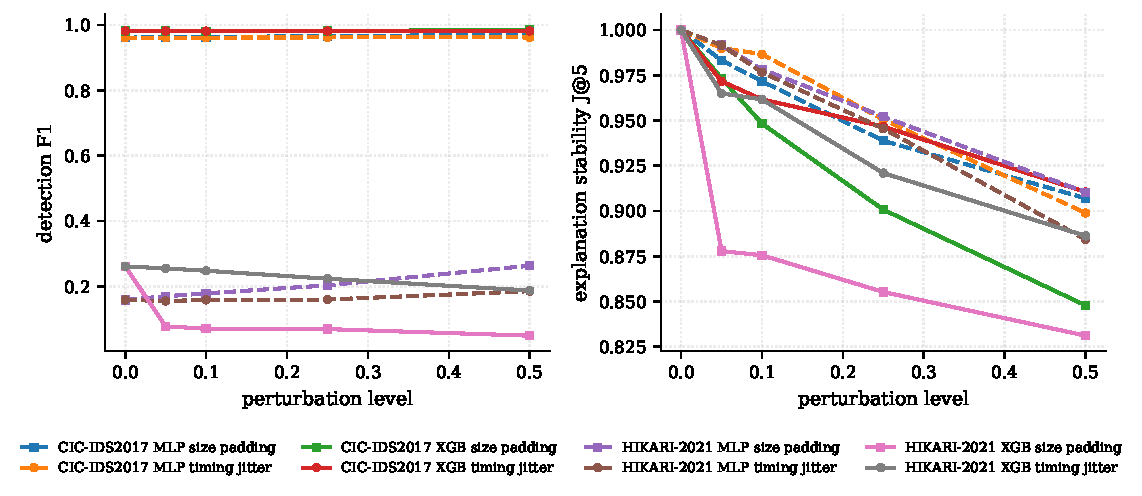
\includegraphics[width=0.62\textwidth]{../figures/fig_robustness.pdf}
\caption{Detection F1 (left) and top-5 explanation stability (right) under increasing timing jitter and size padding.}
\label{fig:robust}
\end{figure}
